\documentclass[conference]{IEEEtran}
\IEEEoverridecommandlockouts
% The preceding line is only needed to identify funding in the first footnote. If that is unneeded, please comment it out.
\usepackage{cite}
\usepackage{amsmath,amssymb,amsfonts}
\usepackage{algorithmic}
\usepackage{graphicx}
\usepackage{textcomp}
\usepackage{xcolor}

\usepackage{fontspec}
\setmainfont{myriad-pro}

\def\BibTeX{{\rm B\kern-.05em{\sc i\kern-.025em b}\kern-.08em
    T\kern-.1667em\lower.7ex\hbox{E}\kern-.125emX}}
\begin{document}

\title{Caching in Named Data Networking\\
}

\author{\IEEEauthorblockN{Christoph Langhans}
\IEEEauthorblockA{\textit{University of Lübeck} \\
Lübeck, Germany \\
christoph.langhans@student.uni-luebeck.de}
}

\maketitle

\begin{abstract}

\textit{Named Data Networking} (NDN) supports the \textit{Internet of Things} (IoT) with features like named-based routing 
and in-network caching. Traditional caching algorithms are ill-suited for energy, storage, and processing-limited IoT devices. 
This paper presents a novel distributed probabilistic caching strategy considering device limitations. We also compare this solution 
to traditional caching strategies in terms of data retrieval and network energy efficiency.
\end{abstract}

\section{Introduction}

In the Internet of Things (IoT), wireless devices interact with their environment and the Internet to support context-aware services. 
As IoT data is smaller and more transient compared to internet content, they require new protocols. Recently, Information-Centric Networking (ICN) has been explored 
for IoT, offering benefits like simplified data retrieval, mobility support, caching, and content-based security \cite{b2, b3, b4}. To address the lack of 
caching strategies for wireless IoT, we introduce pCASTING, a \textit{probabilistic CAching STrategy for the INternet of thinGs} considering data freshness, energy levels, 
and storage capabilities for each network node.

\section{Caching Strategy}

\subsection{Named Data Networking}

NDN is a content dissemination architecture with hierarchical URI-like content names in Interest and Data packets. 
Each NDN Node has three tables: Content Store (CS), Pending Interest Table (PIT), and Forwarding Information Base (FIB) \cite{b9}. 
The node's caching system comprises a caching decision strategy and a replacement policy, determining whether to cache incoming Data 
packets or which packet to replace in a full Content Store, respectively.

\subsection{pCASTING}

In our scenario, a resource-constrained multi-hop wireless network involves $N$ nodes with limited battery energy. Nodes, either fixed 
(e.g., sensors) or mobile (e.g., smartphones), include a set of consumers $C = \{1, ..., N_c\}$, where $N_c < N$ and a producer $P$ generating 
IoT contents with specific freshness. The remaining nodes can cache and forward incoming Data packets. When a node receives a Data packet 
with a matching PIT, the caching decision follows the pCASTING strategy, considering three dynamic attributes related to the device and 
content to calculate the caching probability.

The device-related attributes are \textit{energy level} ($EN$) and \textit{cache occupancy} ($OC$). These values can easily be monitored by the
IoT devices. As a content attribute, we consider the Data \textit{residual freshness} ($FR$). According to NDN, any producer may include in a Data packet a value indicating the freshness $f$ in seconds,
and a timestamp $t_s$ identifying the instant when the information is produced.

We assume that the caching probability is directly (inversely) proportional to each of these parameters. So that for each of the mentioned parameters can be
normalized as $0 \leq EN \leq 1$, $0 \leq OC \leq 1$ where the values $0$ and $1$ mean that the cache or the battery is empty or full, respectively.
The residual freshness can be normalized as $ FR = 1 - \frac{currentTime - t_s}{f}$.
Packets with a negative freshness parameter are considered expired and are not cached at all.

To define the caching probability of a Data packet, we consider a \textit{Caching Utility Function} $F_u$ that takes into account
all of the normalized parameters above. The function can be written as follows:
$$F_u = \sum_{i = 1}^{N_p} w_i g(x_i)$$

where $N_p$ is the number of parameters and the weights $w_i$ assume a value such that $0 \leq w_i \leq 1$ and $\sum_{i = 1}^{N_p} w_i = 1$.
Therefore the weights express the importance of each parameter in the computing of the utility value.

$F_u$ must assume values in the interval $[0 : 1]$ and gives as a result the node's caching probability.

\begin{figure}[htbp]
    \centerline{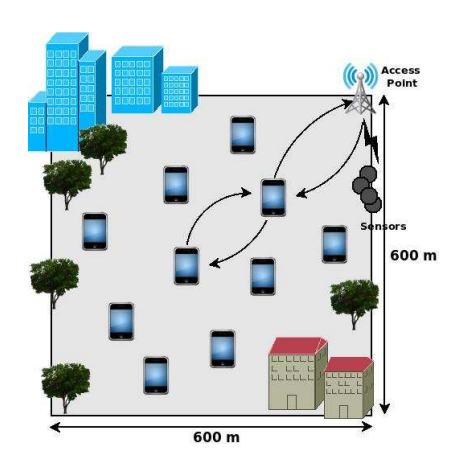
\includegraphics[width=5cm]{fig1.png}}
    \caption{Simulation scenario.}
    \label{fig1}
\end{figure}

\subsection{Experiments}

\begin{table}[htbp]
    \caption{Simulation Settings}
    \begin{center}
    \begin{tabular}{c|c|c|}
    \textbf{Category} & \textbf{Paramter}& \textbf{Value} \\
    \hline
    \textbf{Application} & Data packet size & 512 bytes \\
    & Consumer's freshness & rand(1:10) \\
    & Consumer's update period & 1 minute \\
    & $N_d$ & 5 \\
    \hline
    \textbf{NDN} & CS size & 10 packets \\
    & Routing & controlled flooding \cite{b6}, \cite{b15} \\
    & pCASTING & $w_1 = w_2 = w_3 = 1 / 3$ \\
    & & n = 1 \\
    \hline
    \textbf{Access} & Technology & IEEE 802.11g \\
    & Rx Sensitivity & -83 dBm \\
    & Propagation & Rayleigh \\
    \hline
    \textbf{Scenario} & Area Size & 600m x 600m \\
    & Number of movile nodes & 60 \\
    & Mobility Model & pedestrian \cite{b16} \\
    & Number of Consumers & 1-8 \\
    \end{tabular}
    \label{tab1}
    \end{center}
\end{table}

\begin{figure}[htbp]
    \centerline{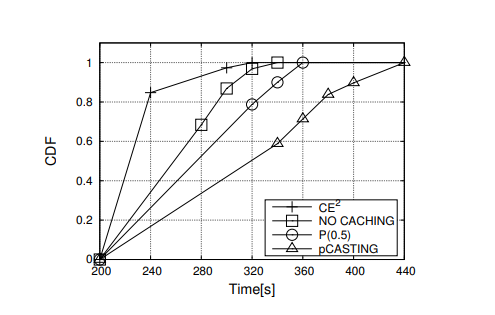
\includegraphics[width=5.5cm]{fig2.png}}
    \caption{CDF of the discharge time of the forwarding nodes.}
    \label{fig2}
\end{figure}

To evaluate the performance of the proposed pCASTING solution we consider a smart city scenario in Fig. 1 representing an urban 
area of size 600m x 600m. A group of sensors deployed in the city periodically generate data for context-aware services. 
An Access Point offers these services to interested consumers. Each service consists of $N_d$ Data packets. The described scenario and the 
pCASTING solution were implemented in the ndnSIM tool \cite{b10}, the reference simulation platform of the NDN research community deployed 
in ns-3 \cite{b18}. Additional information concerning the simulation settings is listed in Table 1.

In the initial analysis, we aim to assess the energy efficiency of pCASTING while ensuring good performance in terms of retrieval delay and 
collected Data. Consumer nodes start with high initial energy while forwarding nodes start with low initial energy. The simulation concludes 
when all forwarding nodes deplete their energy.

As an energy performance metric, we consider the \textit{cumulative distribution function} (CDF) \textit{of the discharge time of the forwarding nodes}.
As indicators of the dissemination performance, we consider three values as listed in Table 2.

We evaluate pCASTING by comparing it to three reference schemes:
Caching Everything Everywhere ($CE^2$), a probabilistic scheme denoted as $P(0.5)$, and a \textit{no caching} scheme.
Results are calculated over ten independent runs and can be examined in Fig. 2 or Table 2, respectively.

\begin{table}[htbp]
    \caption{Data dissemination performance metrics}
    \begin{center}
    \begin{tabular}{c|c|c|c|c|}
    \textbf{Metric} & \textbf{CE$^\text{2}$}& \textbf{No Caching} & \textbf{P(0.5)} & \textbf{pCASTING} \\
    \hline
    \textbf{Cache hit ratio} & $42 \%$ & $0 \%$ & $49 \%$ & $61 \%$ \\
    \hline
    \textbf{Consumers'} & $206$ & $208$ & $217$ & $239$ \\
    \textbf{received data pkts} & & & & \\
    \hline
    \textbf{Data retrieval} & $0.2$ & $0.34$ & $0.18$ & $0.12$ \\
    \textbf{delay[s]} & & & & \\
    \hline
    \end{tabular}
    \label{tab2}
    \end{center}
\end{table}

\begin{figure}[htbp]
    \centerline{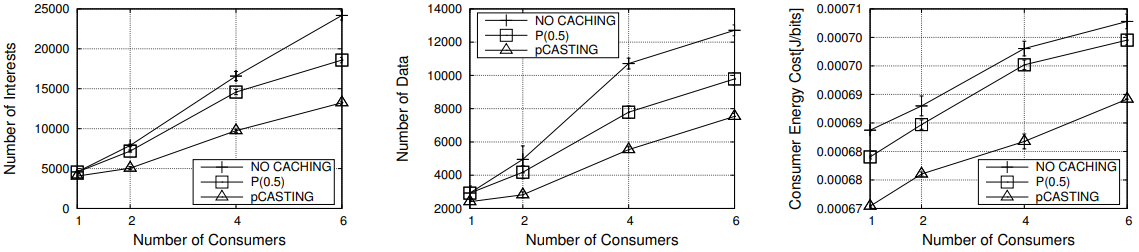
\includegraphics[width=9cm]{fig3.png}}
    \caption{Metrics for retrieval performance analysis}
    \label{fig3}
\end{figure}

In the second experiment, fully charged nodes are monitored for energy consumption over ten minutes. Assessing the caching 
strategy's efficiency from the network perspective involves considering the \textit{number of Interests and Data packets} transmitted. 
From the consumer perspective, efficiency is evaluated by examining \textit{consumer energy costs}, calculated as the average ratio of 
energy spent to correctly received bits.

We compare pCASTING against the \textit{no caching} and $P(0.5)$ scheme. Results are averaged over ten independent runs
and can be examined in Fig. 3.

pCASTING outperforms in all metrics and both experiments, showcasing its energy-aware behavior and probabilistic 
caching decision-making. This approach maximizes content diversity, leading to overall improved performance.


\section{Conclusion}

This paper explores in-network caching in named data wireless IoT networks, introducing the distributed caching scheme, pCASTING. 
This scheme adjusts caching probability based on battery energy level, cache occupancy, and Data packet freshness. Simulation results 
confirm the solution's effectiveness, reducing node energy consumption and ensuring low content retrieval delays. The simplicity of pCASTING's 
caching probability computation allows for easy modification by adding additional parameters.

\begin{thebibliography}{00}
% \bibitem{b1} J. Gubbi, R. Buyya, S. Marusic, and M. Palaniswami, "Internet of Things (IoT): A Vision, Architectural Elements, and Future Directions," \textit{Elsevier Future Generation Computer Systems}, Volume 29, No. 7, 2013.
\bibitem{b2} B. Ahlgren, C. Dannewitz, C. Imbrenda, D. Kutscher, and B. Ohlman, "A Survey of Information-Centric Networking," \textit{IEEE Communications Magazine}, vol. 50, no. 7, pp. 26-36, 2012.
\bibitem{b3} Y. Zhang \textit{et al.}, "ICN based Architecture for IoT - Requirements and Challenges," in \textit{Internet-Draft}, 2014.
\bibitem{b4} M. Amadeo, C. Campolo, A. Iera, and A. Molinaro, "Named Data Networking for IoT: an Architectural Perspective," in \textit{European Conference on Networks and Communications (EuCNC)}, Bologna, Italy, 2014.
% \bibitem{b5} G. Zhang, Y. Li, and T. Lin, "Caching in Information Centric Networking: a Survey," \textit{Elsevier Computer Networks}, vol. 57, no. 16, 2013.
\bibitem{b6} E. Baccelli et al., "Information Centric Networking in the IoT: Experiments with NDN in the Wild," \textit{ACM ICN}, 2014.
% \bibitem{b7} J. Quevedo, D. Corujo, and R. Aguiar, "Consumer Driven Information Freshness Approach for Content Centric Networking," in \textit{IEEE INFOCOM NOM Workshop}, 2014.
% \bibitem{b8} S. Vural et al., "In-network Caching of Internet-of-Things Data," in \textit{IEEE ICC}, 2014.
\bibitem{b9} L. Zhang et al., "Named Data Networking (NDN) Project," PARC, Tech. Rep. NDN-0001, October 2010.
\bibitem{b10} A. Afanasyev et al., "ndnSIM: NDN simulator for NS-3," University of California, Los Angeles, Tech. Rep. NDN-0005, 2012.
% \bibitem{b11} I. Psaras et al., "Probabilistic In-Network Caching for Information-Centric Networks," in \textit{ACM ICN'12}, 2012.
% \bibitem{b12} S. Tarnoi, K. Suksomboon, W. Kumwilaisak, and Y. Ji, "Performance of Probabilistic Caching and Cache Replacement Policies for Content-Centric Networks," in \textit{IEEE LCN}, 2014.
% \bibitem{b13} W. Shang et al., "Securing Building Management Systems Using Named Data Networking," \textit{IEEE Network}, vol. 3, no. 28, 2014.
% \bibitem{b14} L. Wang et al., "Rapid Traffic Information Dissemination Using Named Data," in \textit{ACM NoM'12}, 2012.
\bibitem{b15} M. Amadeo, C. Campolo, and A. Molinaro, "Forwarding Strategies in Named Data Wireless Ad Hoc Networks: Design and Evaluation," \textit{Elsevier Journal of Network and Computer Applications}, 2014.
\bibitem{b16} I. Rhee, M. Shin, S. Hong, K. Lee, and S. Chong, "On the Levy-walk Nature of Human Mobility," in \textit{IEEE INFOCOM}, 2008.
% \bibitem{b17} "Cisco Aironet 802.11a/b/g Wireless Cardbus Adapter, Data Sheet on line at http://www.cisco.com."
\bibitem{b18} "The network simulator-3 (ns-3), http://www.nsnam.org/."
\end{thebibliography}
\vspace{12pt}
\color{red}

\end{document}
